\documentclass[10pt]{beamer}

%%pacotes referentes ao Beamer
%\useoutertheme{split}
%\setbeamertemplate{navigation symbols}{}

%\usetheme{beamertheme}
%\usebeamercolor{beamer-color name}

%\usetheme{Boadilla}
%\usecolortheme{dove}

\usetheme{CambridgeUS}
\usecolortheme{beaver}

% \usetheme{pittsburgh}
% \usecolortheme{dolphin}
%\usecolortheme{dove}
%\usecolortheme{seahorse}

%\usetheme{Montpellier}

%number in figures an tables -- beamer
\setbeamertemplate{caption}[numbered]

%Colocar no description
%[leftmargin=!,labelwidth=\widthof{Turma A}]
	
%pacotes usuais do latex
\usepackage[portuguese]{babel}
\usepackage[utf8]{inputenc}
\usepackage{bm}
\usepackage{graphicx}
\usepackage{subfigure}
\usepackage[round]{natbib}
\usepackage{tikz}
\usetikzlibrary{shapes,arrows}
\usepackage{natbib}
\usepackage{times}
\usepackage{calc} %computes the length of a string
\usepackage{dsfont} %pacote para o 1 estilisado para indicadora
\usepackage{enumerate} %permite fazer uns enumerates diferentes
\usepackage[font=small,labelfont=bf]{caption} %permite colocar um segundo caption
\usepackage{booktabs} % comando \toprule, \midrule e \bottomrule
\usepackage{times} %times new roman font
\usepackage{multirow} %comando \multirow
\usepackage{setspace}
\usepackage{xcolor} %texto colorido
\usepackage{booktabs} %costumized tabs
\usepackage{physics} %absolute value
\usepackage{xcolor}
\usepackage{bigints}


%código para alinhar a esquerda os itens no description
\defbeamertemplate{description item}{align left}{\insertdescriptionitem\hfill}
\defbeamertemplate{enumerate item}{align left}{\insertdescriptionitem\hfill}



%AMS packages
\usepackage{amsmath}
\usepackage{amsfonts}
\usepackage{amssymb}

%Não quebre linhas
\binoppenalty=\maxdimen
\relpenalty=\maxdimen

%Comandos criados por mim
\DeclareMathOperator*{\argmin}{arg\,min}

\DeclareMathOperator*{\argmax}{arg\,max}


\DeclareMathOperator{\espe}{E}

\DeclareMathOperator{\spann}{span}

\DeclareMathOperator{\cov}{Cov}

\DeclareMathOperator{\vari}{Var}

%Informações para o primeiro slide
\date{}
\title[Teste de Hipóteses]{Verificando a normalidade}
\author[Gilberto Sassi]{Gilberto Pereira Sassi}
\institute[IME -- UFBA]{Universidade Federal da Bahia \\ Instituto de Matem\'{a}tica e Estat\'{i}stica\\ Departamento de Estat\'{i}stica }

\begin{document}
	
\tikzstyle{decision} = [diamond, draw, fill=blue!20, 
text width=4.5em, text badly centered, node distance=3cm, inner sep=0pt]
\tikzstyle{block} = [rectangle, draw, fill=blue!20, 
text width=5em, text centered, rounded corners, minimum height=4em]
\tikzstyle{line} = [draw, -latex]
\tikzstyle{cloud} = [draw, ellipse,fill=red!20, node distance=3cm,
minimum height=2em]
	
\begin{frame}{}
	\maketitle
\end{frame}

\section{Verificação da normalidade.}

\begin{frame}{}
 \begin{block}{Objetivo}
 	\begin{itemize}
 		\item Checar se uma variável aleatória contínua $X$ tem modelo de probabilidade normal;
 		\item Vamos usar:
 		\begin{itemize}
 			\item histograma;
 			\item gráfico de quantis;
 			\item teste hipóteses de Kolmogorov-Smirnov;
 		\end{itemize}
 	\item Lembre que só podemos usar o modelo de probabilidade t-Student para o intervalo de confiança e o teste de hipóteses para uma variável aleatória contínua com modelo de probabilidade normal e variância populacional desconhecida.
 	\end{itemize} 
 \end{block}
 

\end{frame}

\begin{frame}{Histograma}

 \begin{block}{Exemplo}
	Devido ao surgimento de um novo vírus, uma empresa começou a vender gel anti-séptico para as mãos. Os frascos conteriam $60ml$ do produto, mas pequenas variações são comuns devido a fatores incontroláveis na produção. Para estudar se a fabricação cumpre os critérios pré-estabelecidos, $20$ frascos foram selecionados aleatoriamente em um certo dia, com os seguintes resultados:
	\begin{table}[htbp]
		\scalebox{0.85}{
			\begin{tabular}{l|cccccccccc}
				\toprule[0.05cm]
				frascos & 1 & 2 & 3 & 4 & 5 & 6 & 7 & 8 & 9 & 10 \\ \midrule[0.025cm]
				conteúdo & 60,8 & 61,5 & 60,5 & 60,9 & 59,9 & 60,2 & 63,9& 59,5 & 59,7 & 62,5 \\
				\midrule[0.05cm]
				frascos & 11 & 12 & 13 & 14 & 15 & 16 & 17 & 18 & 19 & 20 \\ \midrule[0.025cm]
				conteúdo & 59,9 & 60,5 & 60,7 & 55,6 & 57,8 & 58,0 & 57,8 & 61,6 & 59,3 & 62,6\\
				\bottomrule[0.05cm]
			\end{tabular}
		}
	\end{table}
	Verifique se a variável \texttt{conteúdo} tem distribuição normal.
\end{block}	

\end{frame}

\begin{frame}{Histograma}

\footnotesize
\begin{block}{Solução}

\begin{itemize}
	\item A ideia é desenhar o histograma e desenhamos a função de densidade da variável aleatória $N(\bar{x}, s_x)$: se o formatado do histograma e a função de densidade foram iguais, temos indícios de normalidade dos dados;
	\item Para determinar o número de classes, você pode usar a regra de Sturge: $\mbox{Número de faixas} = 1 + \lceil \log_2(n) \rceil$, em que $n$ é o tamanho da amostra.
\end{itemize}


\begin{figure}[htbp]
	\centering
	\caption{Histograma e a função de densidade da distribuição normal.}
	\label{fig:conteudo}
	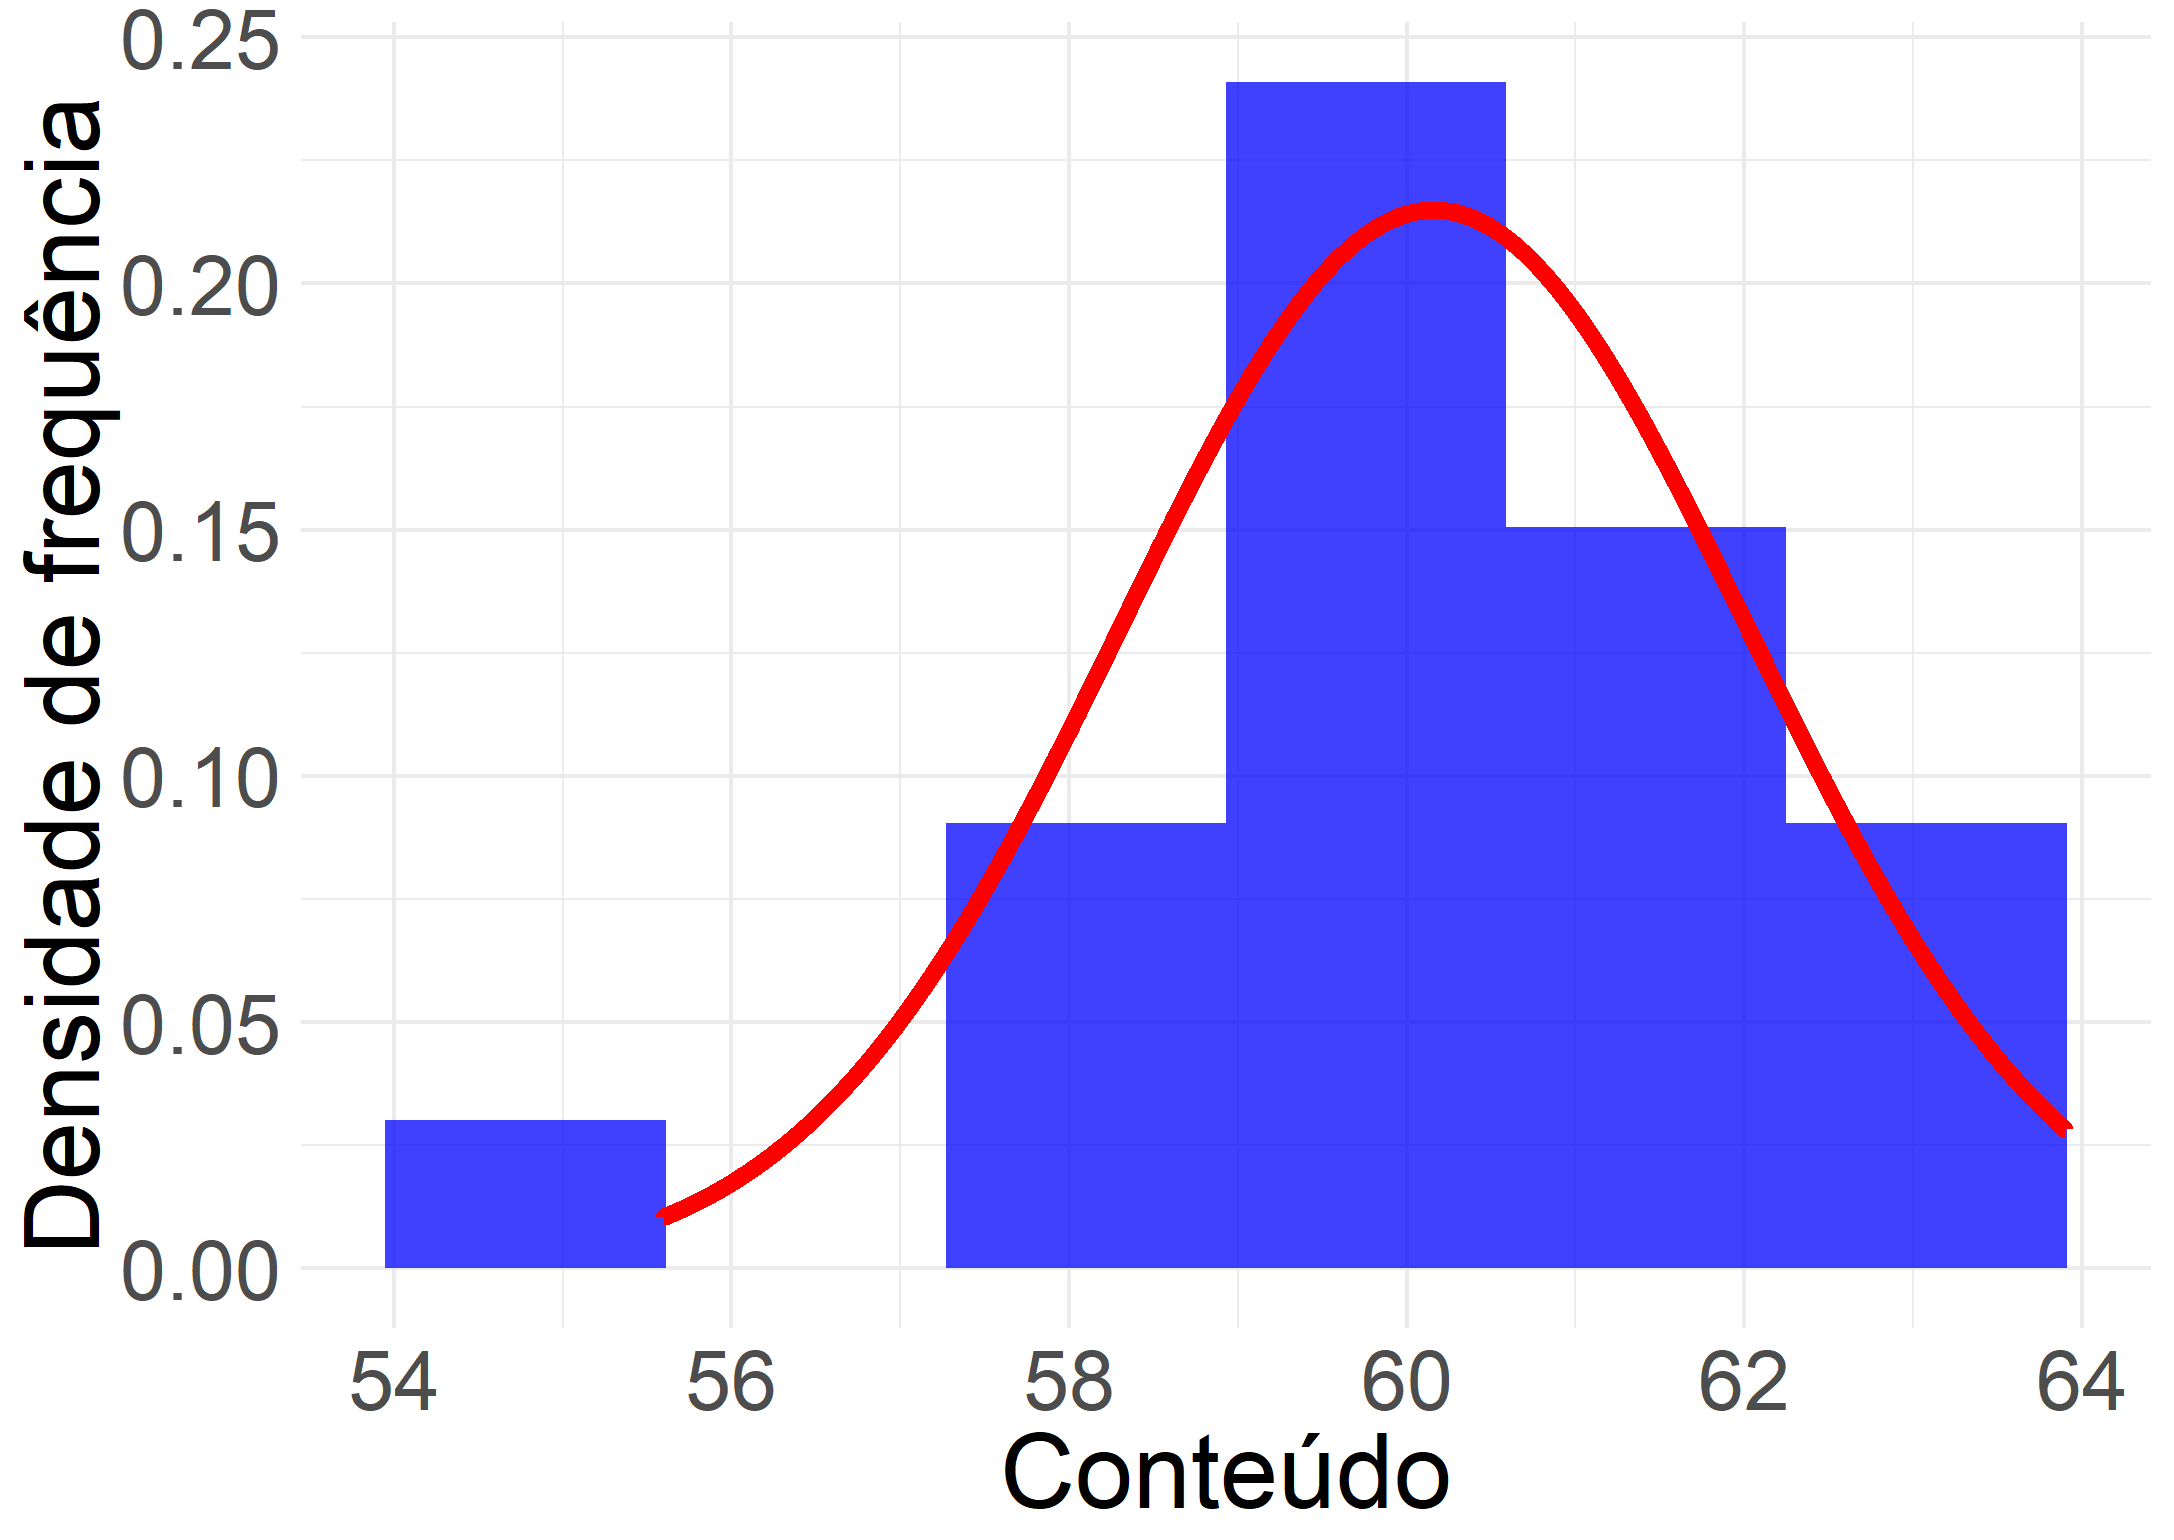
\includegraphics[width=0.35\linewidth]{figures/conteudo.png}
\end{figure}

Pela Figura~\ref{fig:conteudo}, existe indício de normalidade dos dados.

\end{block}
\normalsize

\end{frame}

\subsection{Gráfico de quantis}

\begin{frame}{Gráfico de quantis para duas variáveis}

\footnotesize
\begin{block}{Gráfico de quantis ou Q-Q plot}
	\begin{itemize}
		\item Usamos para verificar se duas variáveis aleatórias têm a mesma distribuição;
		\item Imagine que as amostras de $X$ e $Y$ tem o mesmo tamanho e considere as estatísticas de ordem de $X$ e $Y$:
		\begin{itemize}
			\item $x_{(j)}$: $j$-ésimo menor valor da amostra de $X$;
			\item $y_{(j)}$: $j$-ésimo menor valor da amostra de $Y$;
		\end{itemize}
		Então cada par $(x_{(j)}, y_{(j)}), \ j=1, \dots, n$ é representado por um ponto no plano cartesiano;
		\item Seja $X$ e $Y$ duas variáveis quantitativas com valores observados:
		\begin{align*}
			X:\quad x_1, \dots, x_n,\\
			Y:\quad y_1, \dots, y_m,
		\end{align*}
		em que $m < n$. 
		
		Então cada par $(q_{\left( \frac{j}{m}\right)}, x_{(j)}),\ j=1, \dots, m$, em que $q_{\left( \frac{j}{m}\right)}$ é o quantil de ordem $\frac{j}{m}$ da variável $X$;
		
		\item Se os pontos estiverem próximos da reta de $45^\circ$, temos uma indicação de que as duas variáveis tem o mesmo modelo de probabilidade.
	\end{itemize}
\end{block}
\normalsize

\end{frame}

\begin{frame}{Gráfico de quantis para duas variáveis}


\begin{block}{Exemplo}
	Suponha que desejamos comparar as alturas (em metros) de alunos de ensino médio de duas escolas $A$ e $B$. Uma amostra de $15$ estudantes, foi sorteada em cada um dessas e os resultados são apresentados a seguir:
\begin{table}[htbp]
	\centering
	\caption{Alturas (em $cm$) para as escolas $A$ e $B$.}
	\scalebox{0.7}{
	\begin{tabular}{l|ccccc}
		\toprule[0.05cm]
		\multirow{3}{*}{Escola $A$} & 146,5 & 162,2 & 167,1 & 161,6 & 147,9 \\ 
		&155,6 & 167,4 & 178,8 & 156,1 & 144,1 \\ 
		&165,9 & 165,6 & 164,1 & 161,9 & 169,2 \\ 
		\midrule[0.005cm]
		\multirow{3}{*}{Escola $B$} & 160,4 & 153,1 & 156,3 & 156,8 & 175,4 \\ 
		&154,1 & 155,4 & 160,3 & 163,4 & 174,7 \\ 
		&161,9 & 151,8 & 165,0 & 161,7 & 138,0 \\  \bottomrule[0.05cm]
	\end{tabular}
	}
\end{table}	
\end{block}

\end{frame}


\begin{frame}{Gráfico de quantis para duas variáveis}

\begin{block}{Solução}
Valores ordenados das alturas para as duas escolas $A$ e $B$:
\begin{table}[htbp]
	\centering
	\caption{Alturas (em $cm$) para as escolas $A$ e $B$.}
	\begin{tabular}{l|ccccc}
		\toprule[0.05cm]
		\multirow{3}{*}{Escola $A$} & 144,1 & 146,5 & 147,9 & 155,6 & 156,1 \\ 
		&161,6 & 161,9 & 162,2 & 164,1 & 165,6 \\ 
		&165,9 & 167,1 & 167,4 & 169,2 & 178,8 \\ 
		\midrule[0.005cm]
		\multirow{3}{*}{Escola $B$} & 138,0 & 151,8 & 153,1 & 154,1 & 155,4 \\ 
		&156,3 & 156,8 & 160,3 & 160,4 & 161,7 \\ 
		&161,9 & 163,4 & 165,0 & 174,7 & 175,4 \\ \bottomrule[0.05cm]
	\end{tabular}
\end{table}
\end{block}

\end{frame}


\begin{frame}{Gráfico de quantis para duas variáveis quantitativas}

\begin{block}{Solução}
	No gráfico da Figura~\ref{fig:escolas}, mostramos o gráfico de quantis para as duas variáveis. A linha azul é a reta com inclinação de $45^\circ$ e os pontos estão próximos e em torno desta reta. Logo, as duas variáveis tem o mesmo modelo de probabilidade.
	
	\begin{figure}[htbp]
		\centering
		\caption{Gráfico de quantis para as alturas das crianças na Escola A e na Escola B.}
		\label{fig:escolas}		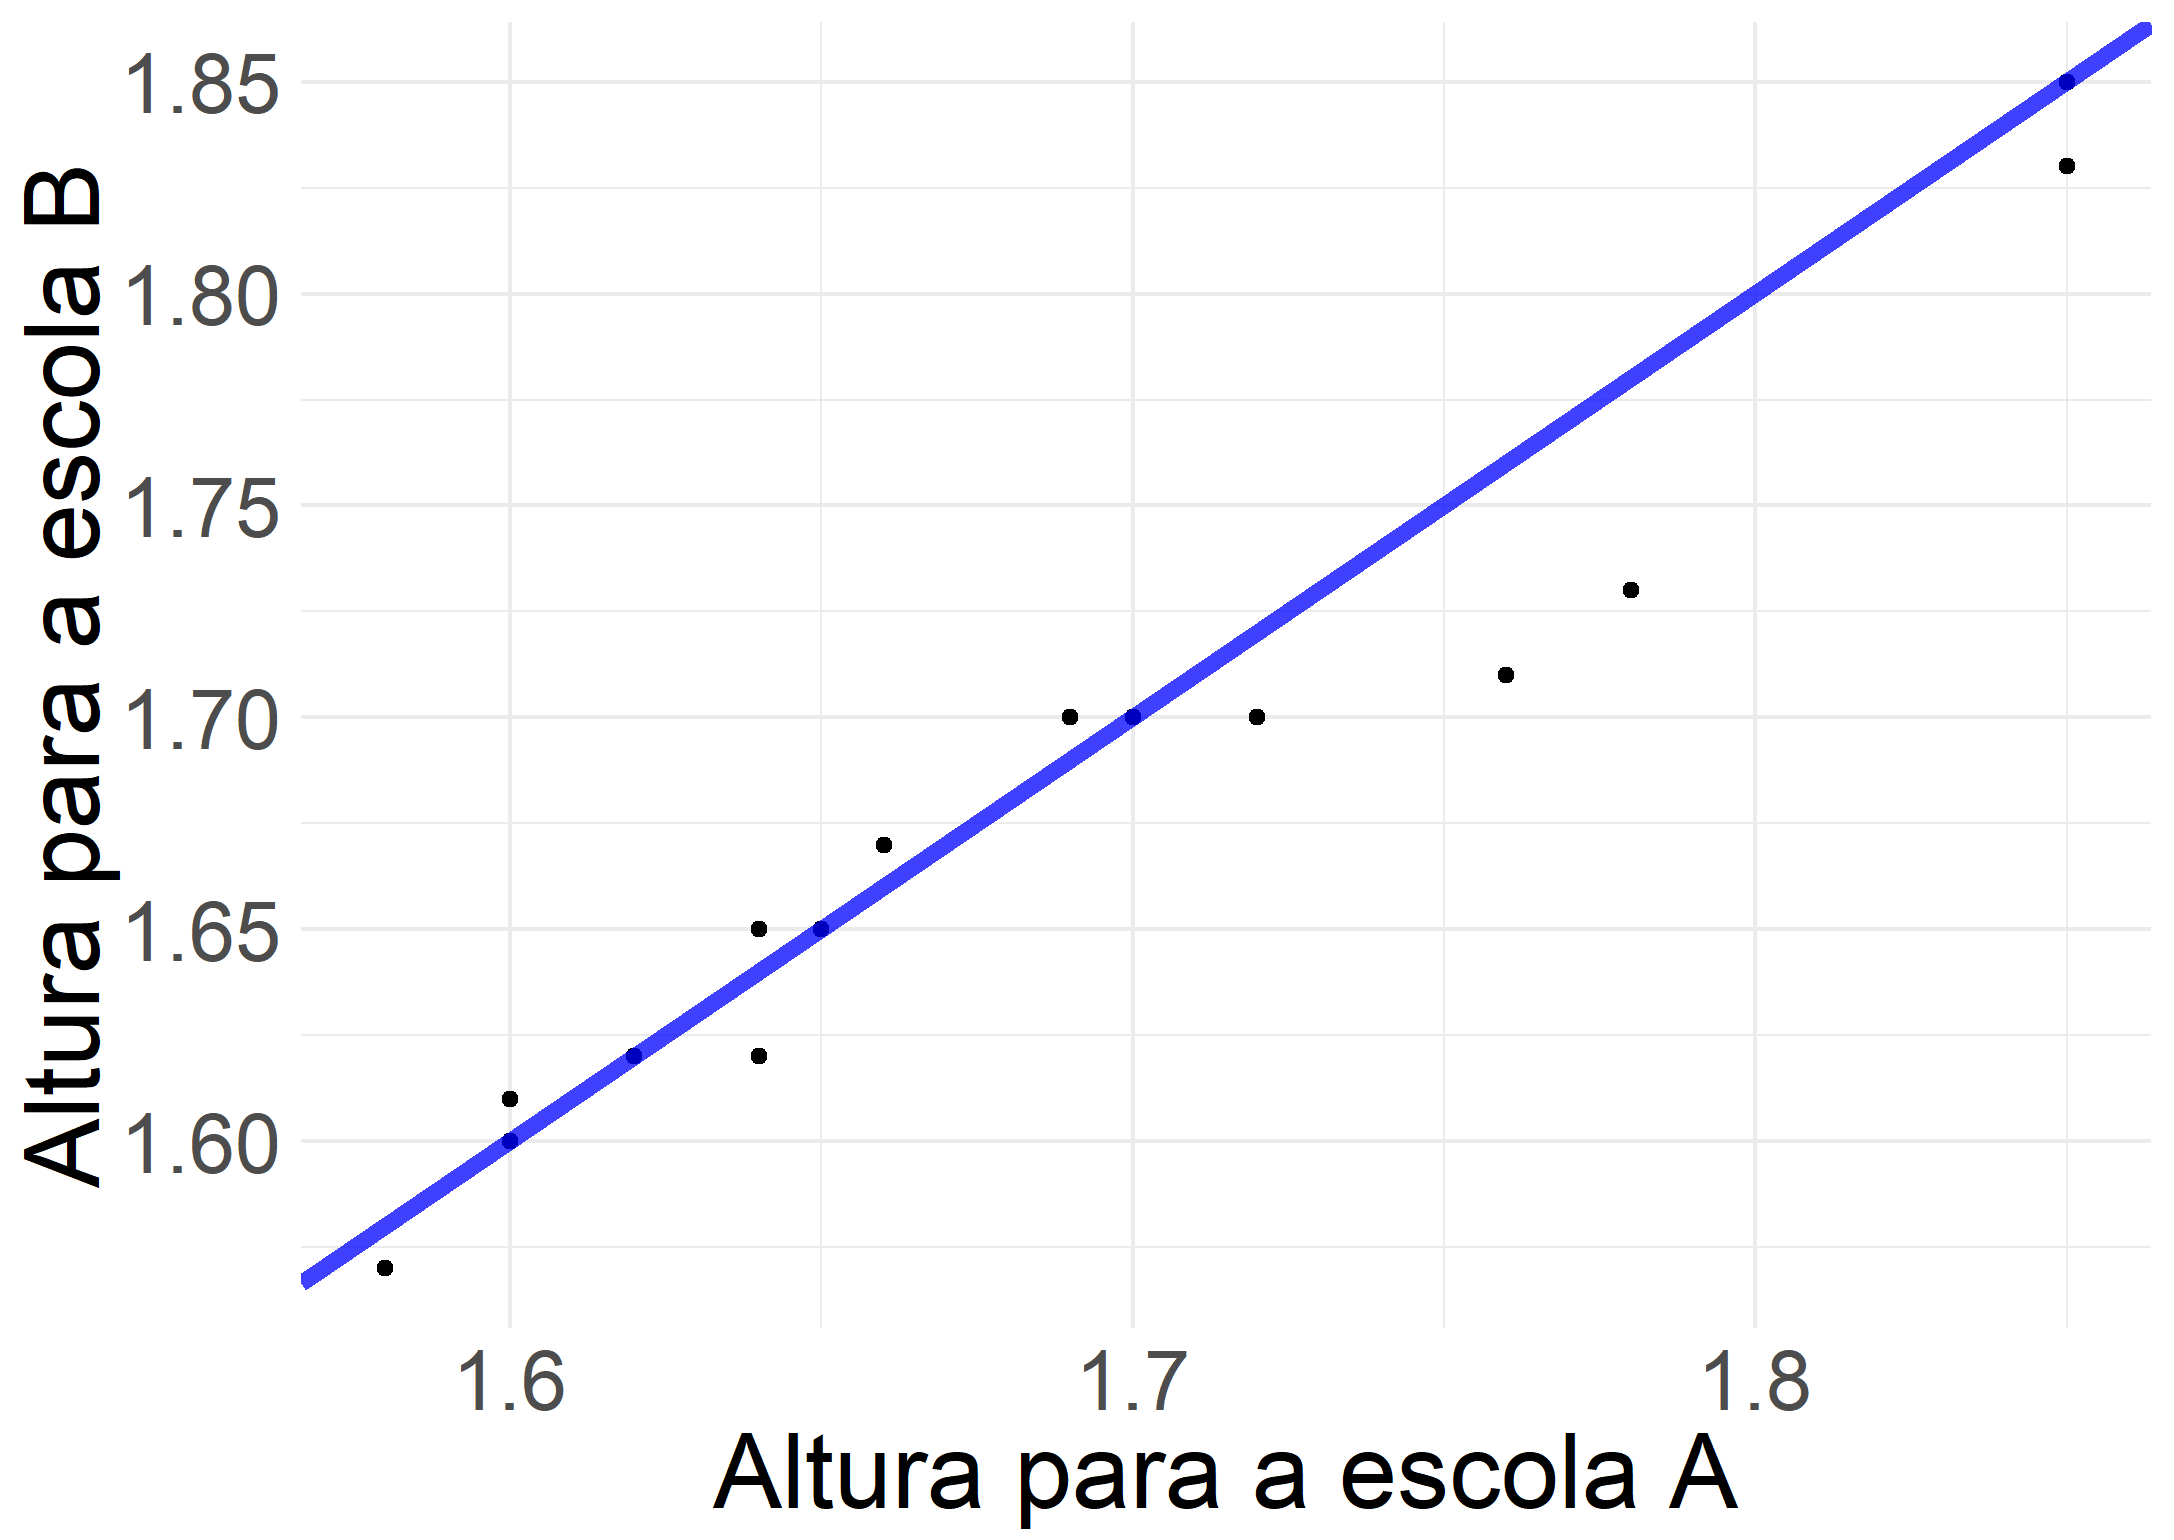
\includegraphics[width=0.4\linewidth]{figures/qqplot.png}
	\end{figure}
\end{block}

\end{frame}

\begin{frame}{Gráfico de probabilidade normal}

Imagine que
\begin{itemize}
	\item $X$ com valores observados $x_1, \dots, x_n$ e estatística de ordem $x_{(1)}, \dots, x_{(n)}$;
	\item Média populacional: $\mu$ e desvio padrão populacional: $\sigma$. Na ausência de $\mu$ e $\sigma$, podemos usar $\bar{x}$ e $s$.
\end{itemize}
\vfill

Considere 
\begin{align*}
z_{(i)} &= \dfrac{x_{(i)}-\mu}{\sigma},\ i=1, \dots, n,\\
\Phi \left( q_{(i)} \right) &=  \dfrac{i - 0,5}{n} ,\ i = 1, \dots, n.
\end{align*}
em que $P(Z < z) = \Phi(z)$ e $Z \sim N(0,1)$.
\vfill

Para cada par $(z_{(i)}, q_{(i)}),\ i=1, \dots, n,$ desenho no ponto um plano cartesiano. Chamamos este gráfico de quantis de \color{red}{gráfico de probabilidade normal.}
\end{frame}

\begin{frame}{Gráfico de probabilidade normal}

\begin{block}{Solução (continuação)}
No gráfico da Figura~\ref{fig:qqnorm}, mostramos o gráfico de quantis de probabilidade normal para a variável \texttt{conteúdo}. A linha azul é a reta com inclinação de $45^\circ$ passando pela origem e os pontos estão próximos e em torno desta reta. Logo, temos indício de que a variável \texttt{conteúdo} tem distribuição normal.
\begin{figure}[htbp]
	\centering
	\caption{Gráfico de quantis: distribuição normal.}
	\label{fig:qqnorm}
	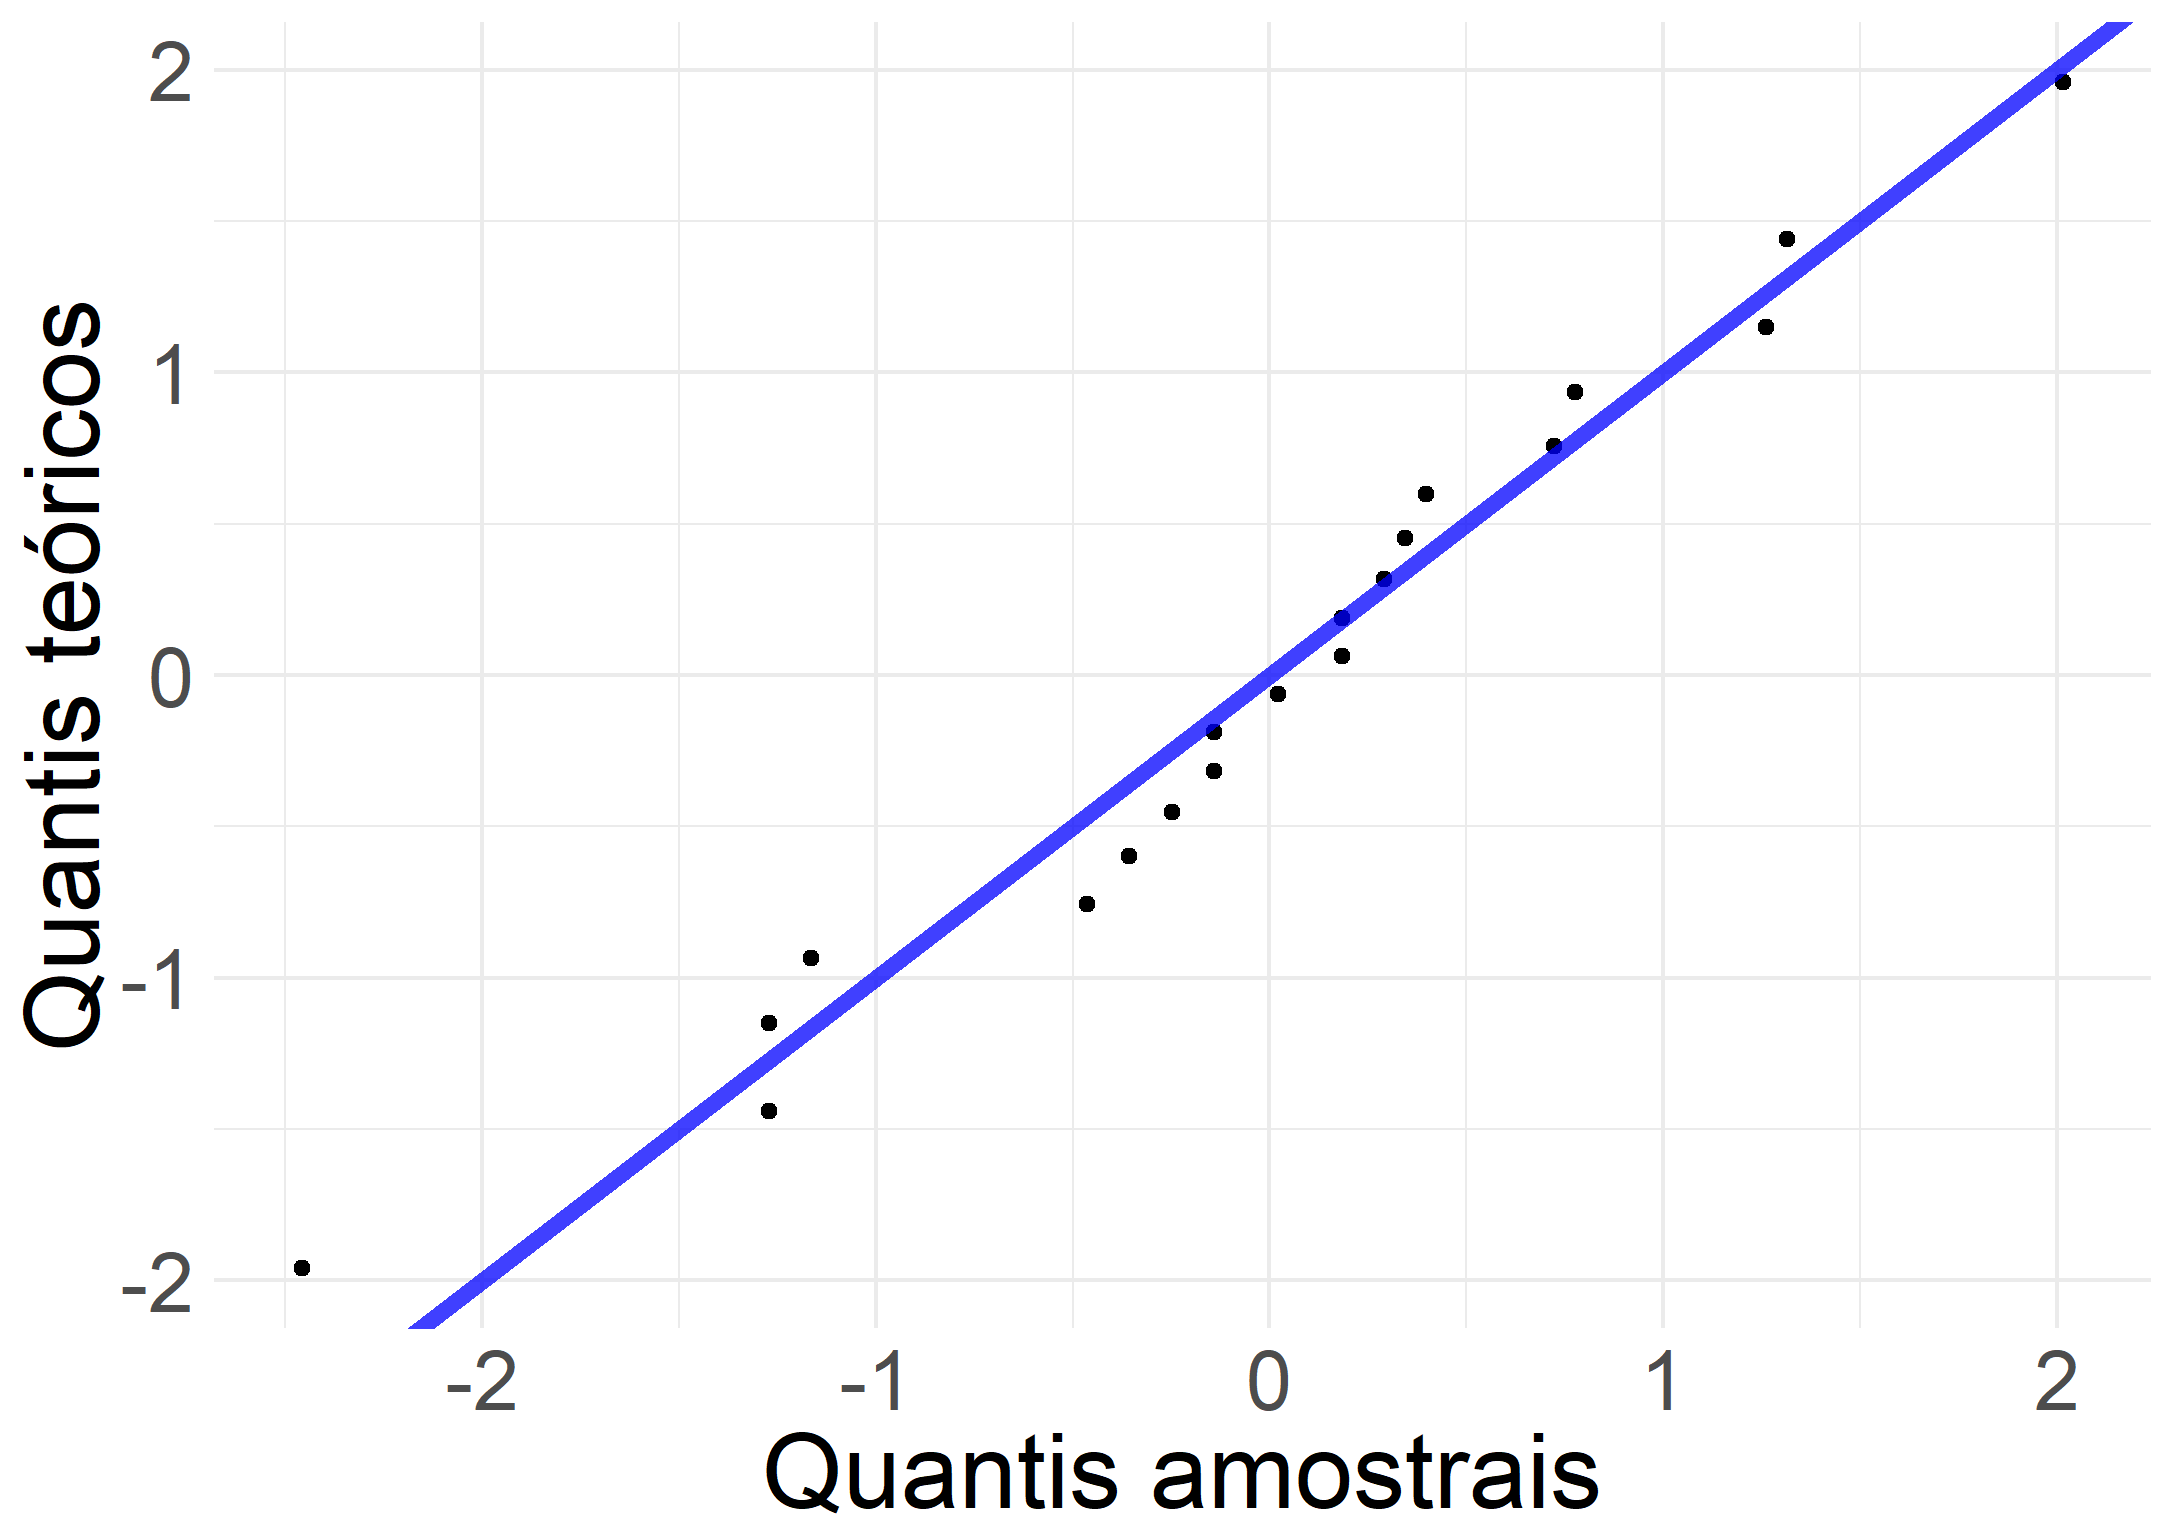
\includegraphics[width=0.4\linewidth]{figures/qqnorm.png}
\end{figure}	
\end{block}

\end{frame}

\subsection{Teste de Normalidade: Kolmogorov-Smirnov}

\begin{frame}{Teste de Kolmogorov-Smirnov}
	\begin{block}{Objetivo}
		Checar se uma variável $X$ tem um determinado modelo de probabilidade. De forma similar, queremos checar se a função de distribuição acumulada $F_X(x)$ da variável é  $F_0(x)$, então temos as hipóteses:
		\begin{align*}
			&H_0: F_X(x)=F_0(x), \forall x,\\
			&H_1: F_X(x) \neq F_0(x), \mbox{para algum valor de }X.
		\end{align*}
	\end{block}

\end{frame}

\begin{frame}{Teste de Kolmogorov-Smirnov}
	\begin{block}{Exemplo}
	Considere uma amostra de 15 equipamentos que foram testados até a sua falha. Verifique se essa variável tem distribuição exponencial com média $\mu=8000$ horas usando o teste de Kolmogorov-Smirnov ao nível de significância $\alpha=5\%$.
	\begin{table}[ht]
		\centering
		\scalebox{0.4}{
			\begin{tabular}{rrrrr}
				\toprule[0.05cm]
				785,17 & 1002,96 & 1373,79 & 1487,74 & 2557,56 \\ 
				4348,16 & 7232,38 & 9491,11 & 9760,40 & 12878,08 \\ 
				15047,12 & 15622,29 & 18460,61 & 20023,98 & 26195,43 \\ 
				\bottomrule[0.05cm]
			\end{tabular}
		}
		\caption{Tempo de vida de um equipamento.} 
		\label{tab:equipamento}
	\end{table}
\end{block}
\end{frame}

\begin{frame}{Teste de Kolmogorov-Smirnov}

\begin{block}{Solução}
	\textbf{Passo 1)} Primeiro vamos estabelecer as hipóteses:
	\begin{align*}
		&H_0: F_X(x) = F_0(x),\\
		&H_1: F_X(x) \neq F_0(x),
	\end{align*}
	em que $F_0(x)$ é a função de distribuição acumulada do modelo exponencial com média $\mu=8000$ horas.
	
	\textbf{Passo 2)} Nível de significância $\alpha = 5\%$. (Tabela tem valores apenas para 5\%, 2\%  e 1\%).
	
	\textbf{Passo 3)} Rejeitamos $H_0$ se $D$ for grande. Ou seja, $RC = \left\{ D \mid D \geq x_c \right\}$, em que 
	\begin{align*}
		D = \max_{1 \leq i \leq n} \lvert F(x_i) -F_e(x_i) \rvert= \max_{1 \leq i \leq n} \lvert F(x_{(i)}) -F_e(x_{(i)}) \rvert = \max_{1 \leq i \leq n} \left\lvert F(x_{(i)}) - \frac{i}{n} \right\rvert.
	\end{align*}
	e $F_e(x) = \frac{N(x)}{n}$ é uma aproximação da função de distribuição acumulada da variável aleatória $X$. 
\end{block}

\end{frame}

\begin{frame}{Teste de Kolmogorov-Smirnov}

\scriptsize

\begin{block}{Solução}
	
	\textbf{Passo 4)} Encontrando o nível de significância: $\alpha = 5\%$.
	\begin{align*}
		\alpha &= P(\mbox{Decidir por }H_1 \mid H_0 \mbox{ é verdadeiro})\\
		&= P(D > x_c \mid H_0 \mbox{ é verdadeiro}).
	\end{align*}
	Para encontrar $x_c$, usamos a tabela X do livro \texttt{Estatística Básica}, e $x_c=0,264$.
	
	\textbf{Passo 5)} Considere $F(x) = 1 - \exp\left(-\frac{x}{\mu}\right),\ x \geq 0$.  Na tabela~\ref{tab:D_exp}, calculamos $\left\lvert F(x_{(i)}) - \frac{i}{n}\right\rvert, i =1, \dots, n,$ e notamos que $D = \max_{1 \leq i \leq n} \left\lvert F(x_{(i)}) - \frac{i}{n}\right\rvert = 0,1613$.
	
		\begin{table}[ht]
		\centering
		\scalebox{0.4}{
		\begin{tabular}{c|c|c|c|c}
			\toprule[0.05cm]
			$i$ & $x_{(i)}$ & $F(x_{(i)}) = 1 - \exp\left( -\frac{x_{(i)}}{\mu} \right)$ & $\frac{i}{n}$ & $\left\lvert 1 - \exp\left( -\frac{x_{(i)}}{\mu} \right) - \frac{i}{n}  \right\rvert$ \\ 
			\midrule[0.05cm]
			1 & 785,17 & 0,0935 & 0,0667 & 0,0268 \\ 
			2 & 1002,96 & 0,1178 & 0,1333 & 0,0155 \\ 
			3 & 1373,79 & 0,1578 & 0,2000 & 0,0422 \\ 
			4 & 1487,74 & 0,1697 & 0,2667 & 0,0970 \\ 
			5 & 2557,56 & 0,2736 & 0,3333 & 0,0597 \\ 
			6 & 4348,16 & 0,4193 & 0,4000 & 0,0193 \\ 
			7 & 7232,38 & 0,5951 & 0,4667 & 0,1284 \\ 
			8 & 9491,11 & 0,6947 & 0,5333 & 0,1613 \\ 
			9 & 9760,40 & 0,7048 & 0,6000 & 0,1048 \\ 
			10 & 12878,08 & 0,8001 & 0,6667 & 0,1334 \\ 
			11 & 15047,12 & 0,8475 & 0,7333 & 0,1142 \\ 
			12 & 15622,29 & 0,8581 & 0,8000 & 0,0581 \\ 
			13 & 18460,61 & 0,9005 & 0,8667 & 0,0338 \\ 
			14 & 20023,98 & 0,9182 & 0,9333 & 0,0152 \\ 
			15 & 26195,43 & 0,9622 & 1,0000 & 0,0378 \\ 
			\bottomrule[0.05cm]
		\end{tabular}
		}
		\caption{Calculando o valor de $D$.} 
		\label{tab:D_exp}
	\end{table}

Como $D = 0,1613 \leq 0,338$ e decidimos por $H_0$, o seja, ao nível de significância $5\%$ decidimos que a variável $X$ tem distribuição exponencial com média $\mu=8000$.
\end{block}

\normalsize
\end{frame}

%\begin{frame}{Solução}
%
%{\small
%	\textbf{Passo 5)}
%
%	Considere $F(x) = 1 - \exp\left(-\frac{x}{\mu}\right),\ x \geq 0$. 
%%	\begin{align*}
%%		F(x) = \begin{cases}
%%		\bigint_{0}^{x} \frac{e^{ -\frac{u}{\mu}}}{\mu} du = 1 - \exp\left(-\frac{x}{\mu}\right), & x \geq 0,\\
%%		F(x) = 0, & x < 0.
%%		\end{cases}
%%	\end{align*}
%	
%	Na tabela~\ref{tab:D_exp}, calculamos $\left\lvert F(x_{(i)}) - \frac{i}{n}\right\rvert, i =1, \dots, n,$ e notamos que $D = \max_{1 \leq i \leq n} \left\lvert F(x_{(i)}) - \frac{i}{n}\right\rvert = 0,1613$.
%	{\scriptsize
%	\begin{table}[ht]
%		\centering
%		\begin{tabular}{c|c|c|c|c}
%			\toprule[0.05cm]
%			$i$ & $x_{(i)}$ & $F(x_{(i)}) = 1 - \exp\left( -\frac{x_{(i)}}{\mu} \right)$ & $\frac{i}{n}$ & $\left\lvert 1 - \exp\left( -\frac{x_{(i)}}{\mu} \right) - \frac{i}{n}  \right\rvert$ \\ 
%			\midrule[0.05cm]
%			1 & 785,17 & 0,0935 & 0,0667 & 0,0268 \\ 
%			2 & 1002,96 & 0,1178 & 0,1333 & 0,0155 \\ 
%			3 & 1373,79 & 0,1578 & 0,2000 & 0,0422 \\ 
%			4 & 1487,74 & 0,1697 & 0,2667 & 0,0970 \\ 
%			5 & 2557,56 & 0,2736 & 0,3333 & 0,0597 \\ 
%			6 & 4348,16 & 0,4193 & 0,4000 & 0,0193 \\ 
%			7 & 7232,38 & 0,5951 & 0,4667 & 0,1284 \\ 
%			8 & 9491,11 & 0,6947 & 0,5333 & 0,1613 \\ 
%			9 & 9760,40 & 0,7048 & 0,6000 & 0,1048 \\ 
%			10 & 12878,08 & 0,8001 & 0,6667 & 0,1334 \\ 
%			11 & 15047,12 & 0,8475 & 0,7333 & 0,1142 \\ 
%			12 & 15622,29 & 0,8581 & 0,8000 & 0,0581 \\ 
%			13 & 18460,61 & 0,9005 & 0,8667 & 0,0338 \\ 
%			14 & 20023,98 & 0,9182 & 0,9333 & 0,0152 \\ 
%			15 & 26195,43 & 0,9622 & 1,0000 & 0,0378 \\ 
%			\bottomrule[0.05cm]
%		\end{tabular}
%		\caption{Calculando o valor de $D$.} 
%		\label{tab:D_exp}
%	\end{table}
%	}
%
%	Como $D = 0,1613 \leq 0,338$ e decidimos por $H_0$, o seja, ao nível de significância $5\%$ decidimos que a variável $X$ tem distribuição exponencial com média $\mu=8000$.
%}	
%
%\end{frame}

\begin{frame}{Teste de Kolmogorov-Smirnov}

\begin{block}{Solução}
Vamos voltar ao exemplo da máquina que enche potes com álcool gel. 
	
	\textbf{Passo 1)} Queremos verificar as seguintes hipóteses:
	\begin{align*}
		&H_0: \mbox{\texttt{conteúdo} tem distribuição normal};\\
		&H_1: \mbox{\texttt{conteúdo} não tem distribuição normal};
	\end{align*}
	
	\textbf{Passo 2)} Nível de significância $\alpha = 5\%$.
	
	\textbf{Passo 3)} Rejeitamos $H_0$ se $D$ for grande. Ou seja, $RC = \left\{ D \mid D > x_c \right\}$, em que $D = \max_{1 \leq i \leq n} \left\lvert \Phi\left( \dfrac{x_{(i)} - \bar{x}}{dp(X)}  \right) - \dfrac{i}{n} \right\rvert$. Ou seja, a região crítica é $RC = \{D \mid D > x_c \}.$

	\textbf{Passo 4)} Usando a tabela X, temos que o valor crítico é $x_c = 0,294$.
\end{block}

\end{frame}

\begin{frame}{Verificando a normalidade dos dados}


	\textbf{Passo 5)} Usando a Tabela~\ref{tab:normalidade}, percebemos que $D =  0,0950 \leq 0,294 = D$ e não rejeitamos $H_0$. Ou seja, ao nível de significância $\alpha=5\%$, a variável aleatória \texttt{conteúdo} tem distribuição normal.
	
	\begin{table}[ht]
		\centering
		\scalebox{0.4}{
		\begin{tabular}{c|c|c|c|c|c}
			\toprule[0.05cm]
			$i$ & $x_{(i)}$ & $z_{(i)} = \frac{x_{(i)} - \bar{x}}{dp(x)}$ & $\Phi\left(z_{(i)}\right)$ & $\frac{i}{n}$ & $\left\lvert \Phi\left(z_{(i)}\right) - \frac{i}{n} \right\rvert$ \\ 
			\midrule[0.05cm]
			 1 & 55,6 & -2,4570 & 0,0070 & 0,0500 & 0,0430 \\ 
			 2 & 57,8 & -1,2716 & 0,1018 & 0,1000 & 0,0018 \\ 
			 3 & 57,8 & -1,2716 & 0,1018 & 0,1500 & 0,0482 \\ 
			 4 & 58,0 & -1,1638 & 0,1222 & 0,2000 & 0,0778 \\ 
			 5 & 59,3 & -0,4634 & 0,3215 & 0,2500 & 0,0715 \\ 
			 6 & 59,5 & -0,3556 & 0,3611 & 0,3000 & 0,0611 \\ 
			 7 & 59,7 & -0,2479 & 0,4021 & 0,3500 & 0,0521 \\ 
			 8 & 59,9 & -0,1401 & 0,4443 & 0,4000 & 0,0443 \\ 
			 9 & 59,9 & -0,1401 & 0,4443 & 0,4500 & 0,0057 \\ 
			 10 & 60,2 & 0,0216 & 0,5086 & 0,5000 & 0,0086 \\ 
			 11 & 60,5 & 0,1832 & 0,5727 & 0,5500 & 0,0227 \\ 
			 12 & 60,5 & 0,1832 & 0,5727 & 0,6000 & 0,0273 \\ 
			 13 & 60,7 & 0,2910 & 0,6145 & 0,6500 & 0,0355 \\ 
			 14 & 60,8 & 0,3448 & 0,6349 & 0,7000 & 0,0651 \\ 
			 15 & 60,9 & 0,3987 & 0,6550 & 0,7500 & 0,0950 \\ 
			 16 & 61,5 & 0,7220 & 0,7649 & 0,8000 & 0,0351 \\ 
			 17 & 61,6 & 0,7759 & 0,7811 & 0,8500 & 0,0689 \\ 
			 18 & 62,5 & 1,2608 & 0,8963 & 0,9000 & 0,0037 \\ 
			 19 & 62,6 & 1,3147 & 0,9057 & 0,9500 & 0,0443 \\ 
			 20 & 63,9 & 2,0152 & 0,9781 & 1,0000 & 0,0219 \\ 
			\bottomrule[0.05cm]
		\end{tabular}
		}
		\caption{Normalidade dos dados.} 
		\label{tab:normalidade}
	\end{table}
	
\end{frame}

\end{document}
